% todo: page limit (= 10); deadline 2/9/2025
% https://www.siam.org/conferences-events/siam-conferences/pp26/submissions/ 
% jb: sections 3, 5, 6, alexis does the rest
%%%%%%%%%%%%%%%%%%%%%%%%%%  example_doublecolumn.tex  %%%%%%%%%%%%%%%%%%%%%%%%%%%%%%%%
%
% This is example_twocolumn.tex, an example file for use with the SIAM LaTeX2E
% Proceedings macros. It is designed to provide two-column output. Please take
% the time to read the following comments, as they document how to use the
% SIAM Proceedings macro files. This file can be composed and printed out for
% use as sample output.
%
% Please submit suggestions for changes to: tex@siam.org.
%
% This file is to be used as an example for style only. It should not be read
% for content.

%%%%%%%%%%%%%%% PLEASE NOTE THE FOLLOWING STYLE RESTRICTIONS %%%%%%%%%%%%%%%

%%  1. There are no new tags.  Existing LaTeX tags have been formatted to match
%%     the SIAM Proceedings style.
%%
%%  2. Do not change the margins or page size!  Do not change from the default
%%     text font or the default text size of 10pt!
%%
%%  3. We recommend that you use BibTeX and siamplain.bst to list your references.
%%     You can use \cite in the text to mark your reference citations and
%%     \bibitem in the listing of references at the end of your chapter. See
%%     the examples in the following file. If you do use BibTeX, please supply
%%     your bib or bbl file with the manuscript file.
%%
%%  4. This macro is set up for two levels of headings (\section and
%%     \subsection). The macro will automatically number the headings for you.
%%
%%  5. No running heads are to be used.
%%
%%  6. Theorems, Lemmas, Definitions, Equations, etc. are to be double numbered,
%%     indicating the section and the occurrence of that element within that 
%%     section. (For example, the first theorem in the second section would be 
%%     numbered 2.1. The macro will automatically do the numbering for you.
%%
%%  7. Figures and Tables must be single-numbered. Use existing LaTeX tags for 
%%     these elements. Numbering will be done automatically.
%%
%%  8. Page numbering is not included in this macro since pagination
%%     will be set by the program committee.
%%

\documentclass[twoside,leqno,twocolumn]{article}

% Comment out the line below if using A4 paper size
\usepackage[letterpaper]{geometry}

\usepackage{siamproceedings}

\usepackage{tikzscale}
\usepackage{pgfplots}
\usepackage{tikz}
\pgfplotsset{compat=newest}
\usetikzlibrary{backgrounds}
\usetikzlibrary{intersections}
\usetikzlibrary{external}
\usetikzlibrary{math}
\usetikzlibrary{positioning}

\usepackage[T1]{fontenc}
\usepackage{amsfonts}
\usepackage{graphicx}
\usepackage{epstopdf}
\usepackage{enumitem}
\usepackage{algorithmic}
\ifpdf
  \DeclareGraphicsExtensions{.eps,.pdf,.png,.jpg}
\else
  \DeclareGraphicsExtensions{.eps}
\fi

% Add a serial/Oxford comma by default.
\newcommand{\creflastconjunction}{, and~}

% Used for creating new theorem and remark environments
\newsiamremark{remark}{Remark}
\newsiamremark{hypothesis}{Hypothesis}
\crefname{hypothesis}{Hypothesis}{Hypotheses}
\newsiamthm{claim}{Claim}

%%Currently, the algorithm title font matches the figure and table title
%%fonts. To make the algorithm title font appear as small caps, uncomment
%%the following code:

%\makeatletter
%\renewcommand{\ALG@name}{\sc Algorithm}
%\makeatother

\usepackage{amsopn}
\DeclareMathOperator{\diag}{diag}

\begin{document}

%
\newcommand\relatedversion{}
% \renewcommand\relatedversion{\thanks{The full version of the paper can be accessed at \protect\url{https://arxiv.org/abs/0000.00000}}} % Replace URL with link to full paper or comment out this line

\pdfinfo{/Author (Alexis Montoison and Jean-Baptiste Caillau)
         /Title (Solving Optimal Control Problems on GPUs)
         /Keywords (optimal control, GPU acceleration, sparse automatic differentiation, interior-point methods, Julia, nonlinear programming, domain-specific language)}

\title{%
  Modelling and optimising control problems on GPUs\thanks{%
  Supported by the FACCTS grant "Detecting Sparsity Patterns in Tapenade for Optimal Quantum Control Applications" of the France-Chicago program. The second author is also funded by a France 2030 support managed by the Agence Nationale de la Recherche, under the reference ANR-23-PEIA-0004 (PDE-AI project).}
}

\author{%
  Alexis Montoison%
  \thanks{%
    Mathematics and Computer Science Division, Argonne National Laboratory, IL, USA.
    E-mail: \email{amontoison@anl.gov}
  }
  \and
  Jean-Baptiste Caillau%
  \thanks{%
    Universit\'e C\^ote d'Azur, CNRS, Inria, LJAD.
    E-mail: \email{jean-baptiste.caillau@univ-cotedazur.fr}
  }
}
\date{\today}

\maketitle

% Copyright Statement
% When submitting your final paper to a SIAM proceedings, it is requested that you include
% the appropriate copyright in the footer of the paper.  The copyright added should be
% consistent with the copyright selected on the copyright form submitted with the paper.
% Please note that "20XX" should be changed to the year of the meeting.

% Default Copyright Statement
\fancyfoot[R]{\scriptsize{Copyright \textcopyright\ 20XX by SIAM\\
Unauthorized reproduction of this article is prohibited}}

% Depending on which copyright you agree to when you sign the copyright form, the copyright
% can be changed to one of the following after commenting out the default copyright statement
% above.

%\fancyfoot[R]{\scriptsize{Copyright \textcopyright\ 20XX\\
%Copyright for this paper is retained by authors}}

%\fancyfoot[R]{\scriptsize{Copyright \textcopyright\ 20XX\\
%Copyright retained by principal author's organization}}

%\pagenumbering{arabic}
%\setcounter{page}{1}%Leave this line commented out.

\begin{abstract}
    We present a fully Julia-based, GPU-accelerated workflow for solving large-scale sparse nonlinear optimal control problems.
    Continuous-time dynamics are modeled and then discretized via direct transcription with OptimalControl.jl into structured sparse nonlinear programs.
    These programs are compiled into GPU kernels using ExaModels.jl, leveraging SIMD parallelism for fast evaluation of objectives, gradients, Jacobians, and Hessians.
    The resulting sparse problems are solved entirely on the GPU using the interior-point solver MadNLP.jl and the GPU sparse linear solver cuDSS, yielding significant speedups over CPU-based approaches.
    % We benchmark the workflow on ...
    % On large-scale instances, we observe a X speedups over CPU-based solvers...
\end{abstract}

% \begin{keywords}
% optimal control, GPU acceleration, sparse automatic differentiation, interior-point methods, Julia, nonlinear programming, domain-specific language
% \end{keywords}

% \begin{AMS}
% 65K10, % Numerical optimization and variational techniques
% 49M37, % Methods of nonlinear programming type
% 65Y20, % Complexity and performance of numerical algorithms
% 68N19  % Other programming techniques (include parallel and GPU programming)
% \end{AMS}

%\tableofcontents
%\listoftodos\relax

\section{Introduction}

Solving large-scale nonlinear optimal control problems is computationally demanding, especially with fine discretizations or real-time requirements.  
While GPUs offer massive parallelism well-suited to these problems, fully exploiting their potential remains challenging due to the complexity of modeling, differentiation, and solver integration.

We present a fully GPU-accelerated workflow, entirely built in Julia~\cite{bezanson2017julia}.
Continuous-time dynamics are discretized with \texttt{OptimalControl.jl}~\cite{Caillau_OptimalControl_jl_a_Julia} into structured, sparse nonlinear programs.  
These are compiled with \texttt{ExaModels.jl}~\cite{shin2024accelerating} into GPU kernels that preserve sparsity and compute derivatives in a single pass, enabling efficient SIMD parallelism.

Problems are solved on NVIDIA GPUs using the interior-point solver \texttt{MadNLP.jl}~\cite{shin2021graph} and the sparse linear solver \texttt{CUDSS.jl}~\cite{Montoison_CUDSS_jl_Julia_interface}, enabling end-to-end acceleration from modeling to solving.

We demonstrate the performance of this approach on benchmark problems solved on GPUs such as the NVIDIA H100 and GH200.

%\textcolor{red}{We also examine generalizations to hybrid systems characterized by discrete-continuous interactions, Pontryagin-based shooting transcriptions, and infinite-horizon or functional programs modeled with \texttt{InfiniteOpt.jl}~\cite{pulsipher2022unifying}. $\rightarrow$ J-B}

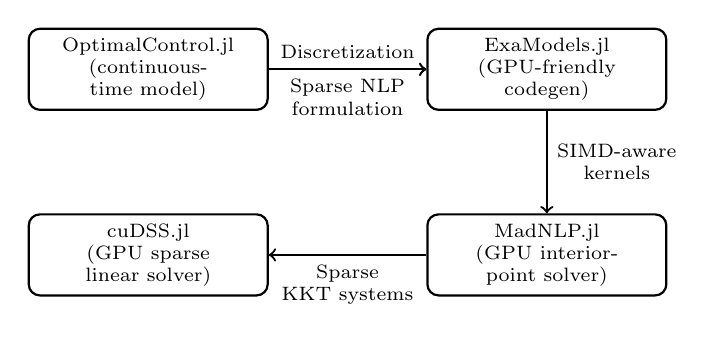
\begin{tikzpicture}[
  node distance=1.3cm and 2cm,
  every node/.style={font=\scriptsize},
  box/.style={
    draw, rounded corners, thick,
    text width=2.8cm, align=center,
    minimum height=0.9cm
  },
  arrow/.style={->, thick}
]

% Nodes
\node[box] (oc) {OptimalControl.jl\\(continuous-time model)};
\node[box, right=of oc] (exa) {ExaModels.jl\\(GPU-friendly codegen)};
\node[box, below=of exa] (mad) {MadNLP.jl\\(GPU interior-point solver)};
\node[box, below=of oc] (cudss) {cuDSS.jl\\(GPU sparse linear solver)};

% Arrows
\draw[arrow] (oc) -- (exa) node[midway, above, align=center] {Discretization};
\draw[arrow] (oc) -- (exa) node[midway, below, align=center] {Sparse NLP\\ formulation};
\draw[arrow] (exa) -- (mad) node[midway, right, align=center] {SIMD-aware\\kernels};
\draw[arrow] (mad) -- (cudss) node[midway, below, align=center] {Sparse\\KKT systems};
\end{tikzpicture}

\section{Background and limitations}

Optimal control problems (OCPs) aim to find control inputs for dynamical systems modeled by ODEs that optimize a given performance criterion.
Direct transcription methods discretize these infinite-dimensional problems into large-scale nonlinear programs (NLPs).
These NLPs exhibit a sparse structure arising from time discretization: each node introduces state and control variables linked by nonlinear equality constraints enforcing the system dynamics.
Second-order methods, such as interior-point solvers, exploit this structure. % for efficient problem solution.

Most existing optimal control toolchains target CPU execution.
For example, CasADi~\cite{Andersson2019} constructs symbolic expressions evaluated just-in-time or exported as C code, typically solved by CPU solvers like IPOPT~\cite{wachter2006implementation} or KNITRO~\cite{byrd2006k}, which rely on CPU linear solvers such as PARDISO~\cite{schenk2004solving}, MUMPS~\cite{amestoy2000mumps}, or HSL~\cite{fowkes2024libhsl}.

Other frameworks such as ACADO~\cite{houska2011acado}, 
\texttt{InfiniteOpt.jl}~\cite{pulsipher2022unifying} (that cleverly leverages 
the modelling power of JuMP~\cite{dunning2017jump}),
Crocoddyl~\cite{mastalli2020crocoddyl}, OCS2~\cite{OCS2} and others
%and AMPL~\cite{fourer1990ampl}
follow the same CPU-centric paradigm.

This CPU focus limits scalability and real-time performance for large or time-critical problems that could benefit from GPU parallelism.
While some libraries provide GPU-accelerated components, none deliver a fully integrated, GPU-native workflow for nonlinear optimal control.

Our work fills this gap with a GPU-first toolchain that unifies modeling, differentiation, and solver execution, addressing the computational challenges of efficient modeling, automatic differentiation, and sparse NLP solving at large scale.

\section{Accelerated direct optimal control with GPU}

When discretized by \emph{direct transcription}, optimal control problems (OCPs) possess an inherent structure that naturally supports SIMD parallelism. 
Consider indeed an optimal control with state $x(t) \in \mathbf{R}^n$, and control $u(t) \in \mathbf{R}^m$. Assume that the dynamics is modeled by the ODE
$$ \dot{x}(t) = f(x(t), u(t)), $$
with $f : \mathbf{R}^n \times \mathbf{R}^m \to \mathbf{R}^n$ is a smooth function. Using a one-step numerical scheme to discretise this ODE on a time grid $t_0, t_1, \dots, t_N$ of size $N + 1$ results in a set of equality constraints. For instance, with a forward Euler scheme, denoting $h_i := t_{i+1} - t_i$, one has ($X_i \simeq x(t_i)$, $U_i \simeq u(t_i)$)
$$ X_{i+1} - X_i - h_i f(X_i, U_i) = 0,\quad i = 0, \dots, N-1. $$
Similarly, a general Bolza cost that mixes endpoint and integral terms as in
$$ g(x(0), x(t_f)) + \int_0^{t_f} f^0(x(t), u(t))\,\mathrm{d}t \to \min $$
can be approximated by
$$ g(X_0, X_N) + \sum_{i=0}^{N-1} h_i f^0(X_i, U_i). $$
Discretising boundary or path constraints such as
$$ b\big(x(0),x(t_f)\big) \leq 0,\quad c\big(x(t), u(t)\big) \leq 0 $$
is obviously done according to
$$ b(X_0, X_N) \leq 0, \quad c(X_i, U_i) \leq 0,\quad i = 0, \dots, N-1. $$
The resulting NLP in the vector $(X_0,\dots,X_N,U_0,\dots,U_{N-1})$
so involves only a few functions (\emph{kernels}), namely $f, f^0$, $g$, $b$ and $c$, that need to be evaluated on many state or control points, $X_i$, $U_i$.
This massive SIMD parallelism allows for a very efficient GPU solving. GPU acceleration thus facilitates real-time and large-scale optimal control computations critical to robotics and autonomous systems as in \cite{pacaud2024gpu}.
% Note that it is also important to exploit the inherent sparsity of the Jacobian of the NLP constraints, see \emph{e.g.} \cite{alexis-xxxx}.
% J-B what do you have in mind with the previous sentence?

%Methods such as multiple shooting or collocation evaluate system dynamics and their derivatives independently across time segments.
%This parallelism, combined with the sparse and structured pattern of derivative blocks, creates a SIMD-like computational workload ideally suited for GPUs.
%Modern GPUs excel at executing many identical computations concurrently, enabling efficient evaluation of ODE right-hand sides and constraint Jacobians across multiple shooting intervals.
%This yields significant speedups, particularly for applications involving multiple rollouts or batched sensitivity analyses, such as Model Predictive Control and reinforcement learning.

% \begin{tikzpicture}[
%   node distance=0.9cm,
%   every node/.style={font=\scriptsize},
%   box/.style={
%     draw, rounded corners, thick,
%     text width=5cm, align=center,
%     minimum height=0.7cm,
%     fill=blue!10
%   },
%   arrow/.style={->, thick, >=stealth}
% ]

% % Nodes
% \node[box] (oc) {Direct Optimal Control Problem};
% \node[box, below=of oc] (discr) {Multiple shooting / Collocation};
% \node[box, below=of discr] (eval) {Parallel evaluation of dynamics \& derivatives \\ (ODE RHS, Jacobians)};
% \node[box, below=of eval] (gpu) {GPU SIMD execution};
% \node[box, below=of gpu, fill=green!10, text width=5cm] (apps) {Applications: MPC, RL, Robotics};

% % Arrows
% \draw[arrow] (oc) -- (discr);
% \draw[arrow] (discr) -- (eval);
% \draw[arrow] (eval) -- (gpu);
% \draw[arrow] (gpu) -- (apps);

% \end{tikzpicture}

\section{GPU programming in Julia}

Julia offers a powerful and flexible environment for GPU programming, providing multiple levels of abstraction to suit different use cases.
The package \texttt{CUDA.jl}~\cite{besard2018juliagpu,besard2019prototyping} provides direct access to NVIDIA GPUs, supporting easy array-based programming as well as explicit CUDA kernel writing and launching.

For vendor-agnostic and portable GPU development, \texttt{KernelAbstractions.jl}~\cite{Churavy_KernelAbstractions_jl} allows writing GPU kernels in Julia that can target multiple backends such as CUDA (NVIDIA), ROCm (AMD), oneAPI (Intel), and Metal (Apple).

This ecosystem leverages the LLVM compiler infrastructure and vendor APIs to generate efficient native GPU code directly from pure high-level Julia code.
It allows users to exploit GPUs without requiring any knowledge of GPU programming.
For instance, \texttt{ExaModels.jl} builds on \texttt{KernelAbstractions.jl} to automatically generate specialized GPU kernels for parallel evaluation of ODE residuals, Jacobians, and Hessians needed in optimal control problems.

We build on this ecosystem to create a complete GPU-accelerated toolchain spanning modeling, differentiation, and solving.

\section{A Julia-based GPU optimization stack}

Building on this GPU programming foundation, we developed a fully Julia-native workflow for modeling and solving ODE-constrained optimal control problems (OCPs) with GPU acceleration.

Key components of our stack include:

\begin{itemize}
    \item \texttt{OptimalControl.jl}: a domain-specific language for symbolic expression of OCPs, supporting both direct and indirect formulations, and generating sparse nonlinear programs.
    \item \texttt{ExaModels.jl}: used to model the discretized OCPs as sparse, 
    SIMD-aware representations that preserve parallelism across grid points, compiling symbolic expressions into optimized code runnable on CPUs and GPUs.
    \item \texttt{MadNLP.jl}: a nonlinear programming solver implementing a filter line-search interior-point method, with GPU-accelerated linear algebra support.
    \item \texttt{CUDSS.jl}: a Julia wrapper around NVIDIA’s \texttt{cuDSS} sparse solver, enabling GPU-based sparse matrix factorizations essential for interior-point methods.
\end{itemize}

Together, these components form a high-level, performant stack that compiles intuitive Julia OCP models into efficient GPU code, achieving substantial speedups while maintaining usability.

Our approach offers several advantages:

\begin{itemize}
    \item \textbf{Abstraction}: intuitive problem definition via Julia DSLs without requiring manual GPU programming.
    \item \textbf{Performance}: JIT compilation, SIMD parallelism, and GPU-accelerated sparse linear algebra deliver significant runtime improvements.
    \item \textbf{Portability}: while symbolic modeling and kernel generation are backend-agnostic, the current bottleneck lies in sparse linear solvers which remain CUDA-specific; however, the framework is designed to adapt as compatible components become available.
\end{itemize}

\section{Benchmark problems}

We evaluate our GPU-accelerated stack on a range of classical optimal control problems, including:

\begin{itemize}
    \item The Goddard rocket problem, a classic single-phase trajectory with nonlinear dynamics;
    \item A quadrotor time-optimal control problem;
    \item The three-link swimmer.
\end{itemize}

These problems are sourced from the COPS benchmark suite~\cite{bondarenko2000cops} and available through the Julia packages \texttt{COPSBenchmarks.jl} and \texttt{CTBenchmarks.jl}.

We compare GPU and CPU performance,
% including against CPU solvers like IPOPT through CasADi,
to assess both raw speedups and the effect of GPU-aware sparsity and parallelism on solver performance.

\section{Alternative tools}

Several Julia packages support optimization over infinite-dimensional spaces.  
For example, \texttt{InfiniteOpt.jl} extends JuMP to express models involving measures, function-valued variables, and continuous domains, with applications to PDE-constrained or stochastic programs.  
However, its emphasis is on symbolic modeling and problem transcription, rather than on GPU-parallel execution.

In contrast, our stack \texttt{OptimalControl.jl}, \texttt{ExaModels.jl}, \texttt{MadNLP.jl}, and \texttt{CUDSS.jl} targets direct OCP formulations transcribed into large-scale sparse NLPs, solved natively on GPUs.

These two approaches are complementary: \texttt{InfiniteOpt.jl} enables high-level modeling for function space problems, while our stack delivers efficient GPU execution for structured, time-discretized OCPs.

\section{Discussion}

Julia’s combination of high-level abstractions, metaprogramming, and GPU compiler infrastructure makes it uniquely suited for building performant yet expressive tools for optimal control.  
Our results show that leveraging parallelism in both model structure and solver internals unlocks substantial speedups, enabling new applications in learning, robotics, and embedded optimization.

% This GPU-based stack allows for large numbers of rollout or sensitivity evaluations in parallel, which is particularly valuable in adaptive MPC, policy learning, or hardware-in-the-loop planning.  

Future extensions include support for multi-GPU execution, as well as tighter integration with differentiable programming workflows.
% MadNCL, MadIPM, HybridKKT, etc...

Overall, the synergy between Julia’s GPU tools and the SIMD structure of direct optimal control yields a powerful solution for solving challenging OCPs at scale.

% Plan
% Introduction -- Context
% controle optimal ODE / direct methods / NLP optim structuré / méthodes indirectes?
% Justification GPU -- first GPU implementation OC / structure adaptée au GPU (massivement SIMD avec la grille)
% Sparsity + SIMD --> large-scale GPUs
% Other tools (CASADI / Ipopt / HSL) but Python and CPU audience (abstraction level -- building blocks?)
% How to handle sparsity on GPU? AD (DSL examodels) + LA (CUDSS.jl)
% Julia is relevant (compilation / metaprog / GPU / PORTABILITY / high-level / efficient)
% KernelABstractions.jl (kernels paramétrique grille)
% OC.jl -> ExaModels.jl -> MadNLP.jl -> CUDSS.jl
% benchmarks
% Benchmarking -- Goddard - quadrotor - swimmer (COPS?)
% GH200 -- 480GB VRAM -- CPU vs GPU
% Casadi + Ipopt gain?
% InfiniteOpt.jl vs OC.jl on CPU

\small
% \bibliographystyle{abbrvnat}
\bibliographystyle{siamplain}
\bibliography{abbrv,main}
\end{document}
